\documentclass[conference]{IEEEtran}
\IEEEoverridecommandlockouts
% The preceding line is only needed to identify funding in the first footnote. If that is unneeded, please comment it out.
\usepackage{cite}
\usepackage{amsmath,amssymb,amsfonts}
\usepackage{algorithmic}
\usepackage{graphicx}
\usepackage{textcomp}
\usepackage{xcolor}
\usepackage{multirow}
\usepackage{rotating}
\usepackage{mdframed}
\usepackage{hyperref}
\usepackage{tikz}
\usepackage{makecell}
\usepackage{tcolorbox}
\usepackage{amsthm}
%\usepackage[english]{babel}
\usepackage{pifont} % checkmarks
%\theoremstyle{definition}
%\newtheorem{definition}{Definition}[section]

\usepackage{listings}
\lstset
{ 
    basicstyle=\footnotesize,
    numbers=left,
    stepnumber=1,
    xleftmargin=5.0ex,
}

%SCJ
\usepackage{subcaption}
\usepackage{array, multirow}
\usepackage{enumitem}

\def\BibTeX{{\rm B\kern-.05em{\sc i\kern-.025em b}\kern-.08em
    T\kern-.1667em\lower.7ex\hbox{E}\kern-.125emX}}
\begin{document}

%\IEEEpubid{978-1-6654-8356-8/22/\$31.00 ©2022 IEEE}
% @Sune:
% Found this suggestion: https://site.ieee.org/compel2018/ieee-copyright-notice/
% I have added it - you can see if it fulfills the requirements

%\IEEEoverridecommandlockouts
%\IEEEpubid{\makebox[\columnwidth]{978-1-6654-8356-8/22/\$31.00 ©2022 IEEE %\hfill} \hspace{\columnsep}\makebox[\columnwidth]{ }}
                                 %978-1-6654-8356-8/22/$31.00 ©2022 IEEE
% copyright notice added:
%\makeatletter
%\setlength{\footskip}{20pt} 
%\def\ps@IEEEtitlepagestyle{%
%  \def\@oddfoot{\mycopyrightnotice}%
%  \def\@evenfoot{}%
%}
%\def\mycopyrightnotice{%
%  {\footnotesize 978-1-6654-8356-8/22/\$31.00 ©2022 IEEE\hfill}% <--- Change here
%  \gdef\mycopyrightnotice{}% just in case
%}
      
\title{Group Report Template\\
}

\author{
    \IEEEauthorblockN{
        Jakub Ratajík\IEEEauthorrefmark{1},
        Kateřina Vácová\IEEEauthorrefmark{1},
        Lara Gutman\IEEEauthorrefmark{1},
        Raluca Elena Mitran\IEEEauthorrefmark{1},
    }
    \IEEEauthorblockA{
        University of Southern Denmark, SDU Software Engineering, Odense, Denmark \\
        Email: \IEEEauthorrefmark{1} \textnormal{\{jarat24,kavac24,lagut24,ramit24\}}@student.sdu.dk
    }
}

%%%%

%\author{\IEEEauthorblockN{1\textsuperscript{st} Blinded for review}
%\IEEEauthorblockA{\textit{Blinded for review} \\
%\textit{Blinded for review}\\
%Blinded for review \\
%Blinded for review}
%\and
%\IEEEauthorblockN{2\textsuperscript{nd} Blinded for review}
%\IEEEauthorblockA{\textit{Blinded for review} \\
%\textit{Blinded for review}\\
%Blinded for review \\
%Blinded for review}
%\and
%\IEEEauthorblockN{3\textsuperscript{nd} Blinded for review}
%\IEEEauthorblockA{\textit{Blinded for review} \\
%\textit{Blinded for review}\\
%Blinded for review \\
%Blinded for review}
%}

%%%%
%\IEEEauthorblockN{2\textsuperscript{nd} Given Name Surname}
%\IEEEauthorblockA{\textit{dept. name of organization (of Aff.)} \\
%\textit{name of organization (of Aff.)}\\
%City, Country \\
%email address or ORCID}

\maketitle
\IEEEpubidadjcol
\begin{abstract}
%%%%%%%%%%%%%%%%%% Max 970 signs without space %%%%%%%%%%%%%%%%%%
% Intro

% Gab
    
% Aim 

% Method

% Results 
The juice manufacturing industry is evolving by integrating Industry 4.0 technologies, aiming to optimize production through intelligent automation. This report presents the design and development of a software architecture tailored for Industry 4.0 machinery in juice production. The proposed architecture ensures 24/7 operational efficiency, scalability, and real-time adaptability. Our approach focuses on the integration of multiple programming languages, databases, and messaging protocols, utilizing microservice-based architectural styles. Through formal verification and validation, we demonstrate the architecture's ability to meet quality attributes such as performance and availability. The results highlight the implementation of continuous production flow with reduced downtime and increased efficiency in juice manufacturing.

\end{abstract}

\begin{IEEEkeywords}
Industry 4.0, Microservices, Quality Attributes, Containerization, Formal Verification
\end{IEEEkeywords}

\section*{Declaration}
    We hereby declare that all sources used in this paper are properly cited and listed. In preparing this paper, we utilized ChatGPT to assist with grammar and style checks. After using this tool, we carefully reviewed the content and take full responsibility for the final output.


\section{Introduction and Motivation}
\color{blue}
%Introduction and motivation to the problem domain.

%Explain why the problem is important and the motivation for solving it.

%Highlight the importance of flexible, dependable architectures in achieving 24/7 operational requirements and adapting to changing production needs.
%\color{red} TODO: Elena
\color{black}

The increasing demand for automation and efficiency in manufacturing has led to the adoption of Industry 4.0 principles across various sectors, including the juice production industry.
In juice production, traditional manufacturing systems often face challenges such as inflexibility in responding to changes in product demand, frequent machine downtimes, the high cost of maintaining legacy systems, and the necessity of running production continuously, with minimal interruptions.
To address these challenges this project aims to design and implement a robust and scalable software architecture that facilitates seamless communication and coordination between production components. Architecture can be defined as the structure, design, and communication between a software system and its components. Therefore, software architecture is usually described as the structure and behavior of a system~\cite{b12}.

The motivation behind this work is to create a flexible architecture with a clearly defined structure that can adapt to changing production needs. This will be achieved by considering quality attributes such as integrability and performance. By incorporating cutting-edge software patterns and strategies, such as event-driven communication and microservices, the architecture will ensure high availability, fault tolerance, and continuous deployment capabilities.

\section{Problem and approach}
%\color{red} TODO: Lara
\color{blue}
%What is the problem* to be solved with the reliable architecture you build, and how will the problem be addressed? The stated problem leads to the stated research question
\color{black}

\subsection{Problem}
There have been numerous problems and ideas that we came across designing and modeling our software architecture. We tried to make it as simple as possible for our customers while also satisfying the industry 4.0 requirements. The main concern was how to make our software architecture adequate to achieve certain quality attributes. As a result of this, we came to our research question.

\subsection{Research Question}
\label{sec:question}
\begin{center}
\textit{"What architectural decisions were made to achieve the quality attributes required for the juice production line?"}
\end{center}

\subsection{Approach}
% I am not 100% happy about this 
%probably have to change 
To address these challenges, our approach focuses on analyzing, designing, and implementing architecture prototypes for the production system components. This architecture must facilitate efficient communication and coordination across the production pipeline to support both routine operations and adaptive production shifts. The architecture will include:

Connectors/Adapters for smooth integration of machinery and other production components.
Coordination Layer to manage interactions, ensuring real-time data exchange and control.
Optimization Layer to regulate production flow and maximize efficiency.
Key system requirements include continuous 24/7 operation, and seamless deployment for incremental updates. The design must incorporate essential quality attributes such as availability, performance, scalability, and modifiability. To achieve this, we will adopt architectural patterns like microservices for modularity, process pairs, and service mash to ensure a better performance in the architecture.

A formal verification and validation process will be employed to confirm that the architectural model satisfies the required quality attributes, addressing both structural and behavioral functionalities. This approach will ensure that the system can maintain operational efficiency and dependability, adapt to production changes dynamically, and support the essential quality properties required for a flexible, automated juice production environment.

\section{Related work}
%\color{red} TODO: Everyone writes about articles, methods, and tools they used 
%\color{blue}
%The related work should review the state of the art consisting of 8-10 papers and should contextualize how this study provides new knowledge to the field. Here, you can combine the work of scientific methods.

%- Review state-of-the-art architectures in Industry 4.0, focusing on examples of middleware systems, message bus integration, and modular robotic components.

%- Discuss the gaps in these systems regarding real-time performance and flexibility, and justify how your approach improves upon them.
\color{black}

The implementation of Industry 4.0 in manufacturing environments has spurred research into flexible, scalable, and interoperable software architectures. Microservice-based architectures have gained popularity in this domain due to their modularity and capacity to manage diverse system components independently. The mentioned studies have demonstrated that microservices are particularly effective in supporting the continuous deployment of software, facilitating frequent updates without disrupting overall system functionality. 

%For instance, Vivek Basavegowda Ramu's (2023) microservice architecture has been shown to greatly enhance scalability and availability in manufacturing systems by enabling independent deployment and scaling of services, which minimizes the risk of entire system failures and optimizes resource utilization. Research demonstrates that microservices also boost system performance by facilitating efficient inter-service communication and supporting robust load balancing, both essential for maintaining 24/7 operations in high-demand production environments. 

\subsection{Diagrams}
When starting to design the software architecture, the architects have a talk with their stakeholders and capture a set of use cases and user stories that should also be in connection with the right quality attributes, which we will talk about later in the report~\cite{b1}. In addition, when creating microservice software, the architecture would be divided into multiple systems that are connected to each other. Moreover, some of the next steps would be creating the system and subsystem diagram, which can show the whole picture of all of the systems in the architecture and their connections.

Besides the use case and system and subsystem diagram, in our architecture design, we have used the feature model diagram. This type of diagram could help us represent all of the features in our system. It not only represents a set of features but also how they are related to each other and how they can be combined with one another. The feature model diagram is usually represented as a tree-like structure. The root of the structure stands for the context, and its children represent the features. In the diagram, exclusion and inclusion exist. Inclusion means that if one particular feature is present, some other features must be present, too. On the other hand, exclusion means if a particular feature is present, some other features must not be included~\cite{b3}. 

The block definition diagram is used to define blocks in terms of their features and their structural relationships with other blocks. It is a part of the structure diagrams that describe the system hierarchy and the system classification~\cite{b4}. Within a classification hierarchy, a block can specialize in another more general block that allows it to inherit features from the general block and to add new features specific to it. The block describes a set of uniquely identifiable instances that share the block’s definition. A block is defined by the features it owns, which may be subdivided into structural features and behavioral features. Behavioral features define how it interacts with its environment or modifies its state~\cite{b4}. 

Requirements represent a capability or a condition that must or should be satisfied. A requirement may specify a function that a system must perform or a performance condition a system must achieve. The requirements of the model are there to identify the mandatory aspects of the architecture. In addition to that, they are also there to plan, organize, and log activities for verification and validation~\cite{b5}.

State Machine Diagram helps with the verification of our system. Specifies the sequences of states that an object goes through during its lifetime in response to events. It specifies the behavior of objects that must respond to stimulus or whose current behavior depends on their past. Also State-Machine Diagram supports event-based behavior~\cite{b5}. 

\subsection{Implementation}
\subsubsection{Programming languages}
\begin{itemize}
    \item Python: Python is a high-level, interpreted programming language renowned for its simplicity and versatility. It provides access to an extensive collection of libraries, many of which are open-source, making it a popular choice for various applications. Python supports several protocols and tools critical to Industry 4.0, such as MQTT, OPC-UA, and ROS (Robot Operating System), enabling seamless communication and integration in industrial environments. Additionally, it offers robust libraries and frameworks for robotics, including ROS, OpenCV, and OpenNI~\cite{b9}, further solidifying its role in automation and robotics. Python's ability to efficiently handle large datasets makes it particularly suitable for industrial automation, where data processing and analysis are essential~\cite{b10}. Its high readability also facilitates collaboration among engineers~\cite{b10}.
    \item Java: Java is a high-level, object-oriented programming language. It is highly suitable for enterprise-level applications with long-term stability and reliability~\cite{b13}. It is compatible with a wide array of tools and protocols, including NoSQL databases and RESTful APIs, which are essential for building interconnected Industry 4.0 systems~\cite{b13}. Java ensures high scalability and performance, making it an ideal choice for handling the high throughput and low latency requirements of RabbitMQ-based systems~\cite{b13}.
\end{itemize}

\subsubsection{Database}
In terms of data management, the combination of SQL and NoSQL databases is increasingly recognized as crucial for handling the diverse data requirements of Industry 4.0 systems. SQL databases are often preferred for structured, transactional data, while NoSQL databases accommodate high-speed access to unstructured data from IoT sensors and other monitoring devices~\cite{b2}. 

A study by Oliveira et al. demonstrated how SQL is well-suited for consistency and reliability, complex relationships, structured data, and operational databases.

On the other hand, NoSQL fits better with high volume, high velocity, high variety data, horizontal scalability, distributed systems and flexibility, and Schema-less Design. 

By balancing the requirements of consistency and reliability (SQL) against the need for flexibility, scalability, and handling of large, diverse datasets (NoSQL), architects can choose the database type that best fits their application's data handling needs~\cite{b2}.

\subsubsection{Message queue}
In the world of software solutions, a message queue is a way of asynchronous communication between entities that need to share information with each other~\cite{Reagan2017Dec}.

As with other decisions in the design, the use of a message queue impacts the final features of a software architecture.

Implementations of message queues differ in their communication protocol, architecture, and the guarantees they provide~\cite{Fu2020Dec}.

In general, message queues are particularly suitable for loosely coupled architectures, including micro-service architectures~\cite{dossot2014rabbitmq}.
The approach of decoupling systems' parts has some implications on the quality attributes. These include among others:

\begin{itemize}
    \item Availability: In addition to allowing early detection (or prevention) of failures of individual parts by messages, if a failure occurs in one of the subsystems, it does not affect the communication of the remaining parts.
    
    On the other hand, without considering other mechanisms, the message queue becomes a single point of failure, potentially disabling the whole system.
    \item Scalability: Due to the partitioning, each part of the system can be expanded or shrunk as needed. One of the potential reasons might also be the volume of messages flooding the message queue.
    \item Performance: The asynchronous nature of messages allows the individual parts of the system to process messages as required. However, in general, the negative impact on the overall system is outweighed by the message-processing overhead.
\end{itemize}

\paragraph{RabbitMQ~\cite{rabbitmq2024Dec} features supporting availability} \label{par:rabbitmq-availability}

\begin{itemize}
    \item Queue mirroring: for each message queue, RabbitMQ maintains a master node and, in addition to it, additional nodes called slaves that serve as its mirror. All actions are first performed on the master node and subsequently pushed to the mirrors. In case of an error of the master node, it is replaced by a slave maintaining access to the consumer.
    \item Acknowledgments: the consumer acknowledges the broker about receiving each message, allowing a control mechanism to detect the unreachability of the consumer.
    \item Publisher confirms mechanism: each time the publisher submits a message to the message broker, the publisher receives a confirmation about the message reaching the broker. This mechanism facilitates the early detection of message queue errors and allows response measures to be taken.
\end{itemize}

\subsubsection{Containerization}
Containerization provides isolation of software components over shared resources. It is used as a means to deploy solutions on computers. 

Containerization has implications on software architecture in terms of various quality attributes (e.g., deployability, scalability), for the purposes of this paper we report the impact on two of them:
\begin{itemize}
    \item \textbf{Availability} is supported by containerization from several perspectives.
    
    Firstly, due to the isolation offered by the containerization paradigm, it is easier to prevent the propagation of a single container fault to the rest of the system.
    
    Secondly, due to abstraction, a container can be scaled as needed and load balance, which avoids overwhelming a single node and consequent unavailability.
    
    Finally, container management allows containers to be restarted, rollbacked, or updated in the event of an error~\cite{b1}.
    \item \textbf{Performance} depends on the performance of the Container Runtime Engine, but it always has to ask for resources from the host and thus introduces overhead. Compared to widely used virtual machines, however, it improves performance by neglecting startup time and reducing memory requirements for running~\cite{b1}.
\end{itemize}

\subsection{Experiment}
\color{black}
Experiments are a fundamental approach in software engineering to assess the validity of claims, determine under what conditions they hold, and establish a context for recommending specific standards, methods, or tools. They play a crucial role in exploring theories, investigating relationships, validating measures, and evaluating the accuracy of models.

To conduct experiments systematically, a structured process is necessary, typically including the following phases: Scoping, Planning, Operation, Analysis and Interpretation, and Presentation and Packaging. These phases ensure the experiment's objectives are clear, methodologies are robust, and findings are effectively communicated.

Experiments involve two key types of variables: independent and dependent. Independent variables are those that are manipulated and controlled during the study, whereas dependent variables are the outcomes measured to assess the impact of changes in the independent variables. Generally, experiments focus on a single dependent variable to maintain clarity in results interpretation~\cite{b14}.

\subsection{V \& V }
%\color{red} TODO: Elena
%\color{blue}
%what is V\&V?
%why formal Verification and Validation (V\&V) is crucial before implementing a system?
%Discuss the relationships and differences between formal V\&V and the experimental evaluation of the system
%Highlight the need for formal design and analysis, including V\&V, before experimental evaluation (e.g., Software-in-the-Loop (SIL), Hardware-in-the-Loop (HIL))
%Discuss the benefits of using V\&V in system development
\color{black}

Verification and Validation (V\&V) are crucial before implementing a system because as a rule, you should not deploy any code without testing it. The architecture should be examined before we build the system to check to which degree it fulfills its quality attributes, in our case performance and availability. Also it is possible to evaluate architectural decisions concerning their impact on those quality attributes. Architecture evaluation is a cheap way to avoid disaster. Architecture evaluation is the process of determining the degree to which an architecture is fit for the purpose for which it is intended \cite{b20}. 

Strong related to V\&V is how the architectural model is structured: structural and behavior model. The structural model is composed of : 
\begin{itemize}
    \item Informal model: Structural model using function blocks + connectors/ports
    \item Formal model: Network Timed Automaton (NTA) consists of a set of Timed Automata (TA)
\end{itemize}
The behavior model is composed of:
\begin{itemize}
    \item Informal semantics model: State Machine Diagram / Sequence Diagram, etc
    \item Formal semantics model:Timed Automaton
    \cite{b21}
\end{itemize}

In conclusion, we can say that in each case either informal or formal verification makes sure that the models created are correctly structured and meet the requirements of the whole system. On the other side, the validation makes sure that the system operates as intended in practice and meets the specified quality attributes.


\subsection{Quality attributes}
Quality attributes are the individual characteristics of a system that go beyond pure functionality and reflect the fulfillment of the requirements for the system. An important aspect of these attributes is that they must be measurable and verifiable.

Each architecture decision enables or hinders individual quality attributes. Therefore, it is important to understand which attributes of the system are crucial for the stakeholders and respective domain and to keep this in mind during the architecture design. Moreover, making decisions towards supporting one of the quality attributes usually decreases other quality attributes and such trade-offs need to be considered.

\textbf{Availability} is a quality attribute that reflects the ability of the system to be available during its operation. In addition to reliability, this also includes the aspect of whether the system can detect, handle, repair, or recover from errors that occur.

\textbf{Performance} is a property of a system to meet specified timing requirements. When events occur (message, request, clock events) the system, or some elements must respond in time~\cite{b1}.

\textbf{Modifiability} is about change, and our interest in it is to lower the cost and risk of making 
changes. When considering this quality attribute, an architect has to consider what can change, what is the likelihood of something changing, when and who makes the changes and what would be the cost~\cite{b1}.

\textbf{Tactics} is a design decision that influences the achievement of a quality attribute response. The focus of a tactic is on single quality attribute~\cite{b1}.

\textbf{Pattern} describes a design problem that arises in specific design contexts and presents an architectural solution for the problem. Patterns often bundle tactics and frequently make trade offs among quality attributes ~\cite{b1}. 

\color{black}


% Systems are designed as structured sets of cooperating architectural elements to make them understandable and to support a variety of other purposes. Every system has its functional and nonfunctional (quality) requirements. They are different from one another. Quality requirements, or in our case, quality attributes, are well defined. For example, performance has to do with the system's timing behavior,  availability has to do with the system's ability to survive failures, and so forth. "A quality attribute (QA) is a measurable or testable property of a system that is used to indicate how well the system satisfies the needs of its stakeholders beyond the basic function of the system." Quality Attributes are divided into two categories. The first category describes some properties of the system at runtime, such as availability, performance, or usability. The second category describes some properties of the development of the system, such as modifiability, testability, or deployability. The achievement of any can have sometimes positive and sometimes negative effects on the achievement of others. Tactics and Patterns are used to achieve the required quality attribute. Furthermore, a tactic and a pattern are some of the techniques used to fulfill a quality attribute. A tactic is a design that influences the achievement of a certain quality attribute, while a pattern describes a certain problem in the process of fulfilling a qa and the solution to that problem~\cite{b1}.

%In summary, existing research offers valuable insights into the integration of microservices, message buses, hybrid databases, and containerization within Industry 4.0 architectures. However, there is limited work on applying these technologies in the context of juice manufacturing, specifically in systems requiring strict quality attributes like continuous deployability and fault tolerance for 24/7 operations. This study aims to build on the foundational work in Industry 4.0 by applying and adapting these architectural components to meet the specific demands of a juice production environment, bridging gaps in continuous deployment and operational reliability.

\section{Use Case}
%\color{red} TODO: Elena (The text that is there now is wrong - we should be talking about our use case meaning the whole juice production) The use case diagram we did should not be even introduced here
%\color{blue}

%Unfold the problem with a use case and describe what the use case is about.

%- Provide a detailed example illustrating the problem.

%- Serve as the foundation for discussing architectural requirements.

Our juice production system was created with the purpose of building a good software architecture that focuses on quality attributes like performance and availability. It is set in Industry 4.0. We have a system that produces natural orange juice and apple juice. The production line system is formed of 4 main systems: Freezer, Juice Production, Storage, and Production Management. The Freezer system refers to the freezers where our resources (the fruits) are kept. 
This system is formed of 2 other subsystems: Adjusting Freezer Properties, which modifies the temperature of the freezers, and Resource Monitoring which keeps track of how many resources we have to make the juice. 

Next with the help of robots and a conveyor belt, the fruits are sent to the Juice Production system that has the Peeling, Squeezing, and Packing subsystems. Each fruit is checked by a robot to see if it’s overripe, in this case, it is thrown to the trash. If the fruit is not overripe, the peeling robot identifies the type of resource and selects the appropriate peeling tool:\begin{itemize}
    \item Zest Peeler for fruits requiring light peeling.
    \item Skin Peeler for items needing a more thorough peel.
\end{itemize}
 If it’s an apple it would be skin peeled, otherwise, if it’s an orange, the fruit would be zest peeled. If the peeling takes more than 60 seconds, the resource will be thrown into the trash. Otherwise, the system evaluates if the peeling is complete. Not being peeled enough means that the resource will be peeled again. After the peeling is done, the fruit is squeezed, and the juice is then packed. The juice is transported to the storage system. Here the amount of juice is being tracked. Also, the juice is shipped through the Shipping subsystem. 
 
The system that manages all the systems mentioned is the Production Management System. Our juice production line works based on subscription. So, for example, a store can have a monthly subscription for orange juice. These subscriptions are handled by the Management of Subscription subsystem. Production Management is also formed by the Production System Monitoring and Scheduling system. The Production Monitoring System oversees the entire production line, continuously tracking and maintaining up-to-date information on the juice production activities. 



\section{Quality Attributes}


\color{black}
Firstly, one of the quality attributes that we have been focusing on while designing and implementing the Juice factory was availability. Availability refers to the software being ready to carry out its task when you need it. Furthermore, all of the availability tactics are connected with faults. These kinds of faults must be detected or anticipated. The tactic implemented in our architecture would be "Heartbeat", where a periodic message exchange between a monitoring system and a peeling system is being exchanged. The system monitor receives the messages of the processes the peeling system is going through. Not only will the monitoring system know which fault happened, but also when. The way of recovering from this fault would be a redundant spare. One or more duplicate components can step in and take over the work if the primary component fails~\cite{b1}.

Secondly, performance was a quality attribute that we considered important for our software architecture. Operations on computers take time. When events like, for example, messages, requests from users, or other subsystems occur, the system or some parts of the system must respond to them in time. The system is either going to respond to that event, or the processing is going to be blocked for some reason. What's more, the pattern used to reach better performance in the microservice architecture would be the service mesh pattern. This kind of approach allows developers to divide the functionality of the microservice from the implementation, management, and other parts~\cite{b1}. 

In addition, with our experiment, which we talk about more in chapter 7, we created a performance scenario. The source of our experiment was the peeling subsystem that sends a message, to the monitoring subsystem. In this case, the stimulus of our scenario is the message. This message contains the status of the peeling subsystem and the time of when it was sent. One of our main concerns were how long will it take for the message to be delivered from the source to the receiver and how many messages will be sent to the monitoring subsystem in 5 minutes. When it comes to our artifact, it is presented by the whole system. The environment is set in a normal setup. Not only wasn't it overloaded, but more messages were being sent the faster the system became. The response of the scenario was received by the monitoring subsystem. The response was a message containing the status of the peeling subsystem and the time it was sent. The response measure of the system would be the average time of the difference between the time of the arrival and the time the message was sent. In addition, it would get the timestamp of when it arrived, that way we could determine if our architecture achieved the wanted delivery time and if it was performing the way we imagined it. 

Quality attributes define the essential non-functional requirements for our Industry 4.0 software architecture, shaping how effectively the system supports continuous, adaptable, and high-quality production in the juice industry. The selected attributes guide design choices, ensuring that the system not only meets functional requirements but also excels in reliability, performance, scalability, and other operational needs, thus enabling smooth 24/7 operation and continuous deployment capabilities.

These quality attributes collectively ensure that the software architecture can support high-demand, reliable, and secure juice production operations. By prioritizing availability
and performance, the architecture aligns with Industry 4.0 objectives, supporting continuous improvements and adaptation to industry needs.

\section{Design and analysis modeling}
%Based on the course context,  production system requirements, and your use cases,  note down details that could be relevant when defining systems and their respective subsystems.  For example, what components need to work 24/7?  Which parts need to be continuously deployable?
%\color{red} TODO: Lara

%\color{blue}
%- Describe the design and argue for the design decision and how it meets the QASes. Part of the design decision must specify which tactics/patterns are used (provide arguments) and the trade-offs

%- Analyze the design and illustrate the system architecture model, encompassing both structure and behavior, using formal reasoning
\color{black}

In this chapter, we will talk about the design and analysis modeling of our Juice Factory I 4.0 software tool. 
\subsection{Diagrams}
When we were thinking of how our software architecture would look like we thought of microservices. The idea of microservices is to design highly independent services that implement small units of functionality and can interact with each other through interfaces~\cite{b6}. The important services for our software tool are divided into multiple systems and subsystems. Not only would the possibility of the system running 24/7 be easier to implement, but also developers can deploy only certain parts of the system while the other parts are working normally.

In addition, to get a better picture of how the systems would be connected with one another we made a feature model like on the picture. This way we could understand better how they are connected with one another and how would the trace of the information go. Furthermore, we have decided to focus on 2 subsystems in our software architecture, their mutual relationship, and how they interact with one another. 

Apart from these diagrams, we designed a structure model to serve as basis for a component based build-system that provides the benefits. These benefits include clearly visible dependency descriptors between components, uniform build and configuration interfaces, build and deployment processes on component level, and automated component composition~\cite{b11}. 

We have designed a Block Definition Diagram (BDD) for our peeling system. The implemented BDD is a set of relationships between each other. Within our BDD we have blocks that inherit features from previous block so it can do it's job and send it's results to the next block~\cite{b4}. BDD represents a total of function blocks that have an important role in designing out architecture. It is a structured model that can show the trace of information. 

On top of that, we have requirements that check if the information is going well or how fast the information is being delivered from one function block to the next one. More about this in the requirements chapter. 
\subsection{Requirements}
%\color{blue}
%- Link the identified requirements to both the structural model from step and the behavioral models.
\color{black}
We have written down the requirements that should be satisfied when it comes to our chosen system and its connection.
\begin{itemize}
    \item R1: Receive the cleaned resources from the cleaning machine. 
    \item R2: Overripe resources are thrown out. 
    \item R3: Oranges or apples are recognized by the machine.
    \item R4: Skin peeling for apples, zest peeling for oranges.
    \item R5: Resources passed downstream have to be peeled enough.
    \item R6: The peeling process should not take more than 60 seconds per resource piece.
    \item R7: The squeezer robot is notified about the resource being ready, i.e. peeled.
\end{itemize}


While we were writing the requirements for the implementation of our peeling subsystem, we were trying to focus on the availability of the system. If the robots are checking the ripeness of the resource or if it takes more than 60s to peel the resource, we should throw it out and make it available for the next one. 

Not only are we thinking about the availability, but also performance. What's more, it is important to make a time condition for how long it can peel a resource. That way we are tending the system to respond as quickly as possible, not having much of a block time. The process can not proceed if the peeling robot is unavailable. Unavailability is caused by the resource being overripe or the process of peeling is taking too much time. 

Hence, we have implemented 2 requirements, "R2" and "R6", that would manage work requests by reducing the number of requests. The peeling robot throws the overripe resource and does not spend time on it, which increases performance and availability. In addition to that, we made a prioritization of the resources. 

One of the patterns implemented in our architecture that can provide these quality attributes is Service Mash. Service Mash is used in microservice architectures. It addresses application-independent concerns such as interservice communications, monitoring, and security. We have monitoring subsystem which is a sidecar that executes alongside each microservice and handles all interservice communication and coordination.This approach allows developers to separate the functionality—the core business logic~\cite{b1}.

In summary, by implementing these requirements we are trying to make these subsystems work 24/7. If the peeling system is working 24/7, more resources can be peeled, time and money are being saved. In addition, monitoring system can have the whole picture of other systems and how they are functioning 24/7.

\subsection{Implementation}
\color{black}

For this paper, we decided to focus on implementing the software tool only for two subsystems: monitoring and peeling subsystems. 
What's more, while focusing on which software technologies would be the best for our architecture, we had to devote ourselves to the quality attributes that are important for our architecture. 

\subsubsection{Databases}
When it comes to implementing databases in the peeling system, we opted for a more flexible one, which is the NoSQL database (MongoDB). NoSQL databases are more dynamic, unstructured, flexible, and great for large volumes of data. It is well-equipped to handle huge and diverse datasets and uses fewer resources to ensure data integrity and consistency. 

This means that the system guarantees availability, ensuring that data requests will receive a response, even if it is not the most up-to-date or accurate. The system remains operational, but it may not always reflect the most current state of the data. Not only does it secure availability, but it also makes the system faster and allows better performance. It is able to provide the system to work 24/7, even if there are small glitches. 

However, when it comes to the monitoring system, we took a different approach. SQL (PostgreSQL) seemed like a better option. SQL is a well-structured relation database that guarantees that once a transaction is committed, it will remain so, even in the event of a system failure. Ensures that transactions occur independently of each other. If any part of the transaction fails, the entire transaction is rolled back, leaving the database in its original state~\cite{b2}. The monitoring system stores different kinds of data like subscriptions, resources, users, etc. 

In addition, this way, security and availability are certain. They contribute to fault prevention by ensuring transaction consistency, which aligns well with high availability demands in a monitoring system where data integrity is critical~\cite{b1}.

\subsubsection{Message queue}
In the case of the proposed architecture, the partitioning of the individual systems into separate units leads to the necessity of using a way in which the individual subsystems can communicate.

The choice of the part of our architecture to be implemented reflects our attention to the chosen quality attributes, namely availability.

Therefore, the key role of this component is to ensure communication between the monitoring system and the other components of the production line. Most messages passing through this communication channel, therefore, contain information regarding the current components' state, their performing process, or an occurred error. 

We have chosen to use RabbitMQ as the appropriate message queue for our case. The main reason includes our requirement for an availability quality attribute, which RabbitMQ supports as discussed in~\ref{par:rabbitmq-availability}.

However, it must be noted that there are messaging tools that achieve far better results in other metrics and, thus, in the case of emphasis on other quality attributes.

For example, Apache Kafka~\cite{garg2013apache}, which achieves significantly higher throughput in the existing benchmark~\cite{Fu2020Dec}. In the case of a large number of messages, it would therefore be worth considering prioritizing higher throughput and thus enabling performance. However, in the case of our production line, the amount of messages is relatively small (compared to streaming services using Kafka), and the need for availability, therefore, outweighs.
Furthermore, RabbitMQ, unlike Apache Kafka, supports message priority, which is important in our system since a message about an error in one of the subsystems is more important than a message about the resource-peeling completion.


%% By  containerizing  different  components  of  your  system,  you  aim  to  enhance  theportability, scalability, and maintainability of your software, allowing for more seamless deployment,scaling, and development processes

\subsubsection{Programming languages}
For the peeling subsystem, Python was chosen as the programming language. This decision was primarily due to Python's extensive support for various robotics frameworks, which is unmatched by other programming languages. Python's flexibility and widespread adoption in the robotics community made it an ideal choice for developing a platform to communicate with the peeling robot.

However, the decision for the monitoring subsystem was less straightforward. For example, while using C instead of Java could provide higher efficiency and better control over system resources, Java offers advantages such as an official RabbitMQ client library and suitability for parallel systems, making it a strong contender for the task.

\section{Formal verification and validation }
%\color{red} TODO: Elena
%\color{blue}
%- Formalize the system requirements, including functional properties associated with quality attributes. 

%- Perform formal verification and simulation to determine if the system meets the specified requirements. Provide the V\&V results, along with any counter-examples

%-Which/what parts of your system design will be formally specified, verified and validated? why and how?
%-What are the timing constraints of your architecture models?
%-Identify and define the type of constraint, i.e., event-chain- or event-constraint regarding your system design
\color{black}

We chose to formally specify, verify, and validate the peeling and monitoring part of our system design because the performance can be evaluated through the messages sent from the peeling system to the monitoring.
In this chapter, we are presenting the formal V\&V so the Timed Automata we created in UPPAAL, and our experiment.
\subsection{Architectural Structure \& FSM (Finite-State Machine/ Finite-State Automaton) \cite{b7}}
One part of the model-checking overview is made of the architectural structure (function blocks) and operational behaviors (FSM-based notations).
%Elena
FSM (Finite-State Machine/ Finite-State Automaton) is an abstract machine that can be in one of a finite number of states. It can only be in one state at a time. A state is a description of the status of an FSM that is waiting to execute a transition. A transition is when, in a finite state machine, it goes from one state to another when initiated by a triggering event or conditions. The transition is a set of actions that can be executed when a certain condition is fulfilled.   

Timed Automata (TA) is FSM extended with clock variables.  

We have decided to represent our Peeling System in Timed Automata. With help from drawing our FSM, we have accomplished implementing it in UPPAAL. Our system has 4 TA: "PeelingMachine", "PeelingCheckerSensor" and "Monitoring" and "ConveyorBelt".  

The "PeelingMachine" represents the core of the peeling System which begins with the state "Idle",  because it is the beginning of the peeling process. 

In UPPAAL, we used guards, synchronization (sync), and update. The guard acts like a condition; in our example, we used time $\geq 60$ to check if the peeling takes too long. In this case, the fruit is thrown into the trash, so in location, throw out resources. We could have also used invariants. An invariant is similar to a condition in which, if it is violated, the system must leave the location. So, invariants can be used to limit the time that the systems can stay in a location.

Synchronization can be of two types: binary synchronization declared like chan its\_enough and broadcast synchronization declared like broadcast chan. In the case of it is enough, we check if the fruit is peeled enough. Its\_enough! is emitting, and its\_enough? is receiving on the same channel, so these edges are in different processes, but they synchronize. We could also make use of urgent and committed locations, but it was not necessary. 

Model Checking explores all possible transitions out of system states that satisfy the initial condition and ensures that all other executions satisfy the property. In the process of model checking and verification, we are looking into the safety and liveness of the system. Safety implies that "nothing bad ever happens," and liveness means "something good eventually happens." 

Some of our queries are: 
\begin{itemize}
\item \texttt{A [] not deadlock}
where we are checking that our system never reaches deadlock. The next one would be  

\item \texttt{E <> time $\geq$ 60} 
where we are checking if there is a possibility of the system peeling a resource for more than 60 seconds.  

\item \texttt{A [] not (PeelingMachine.resource == PeelingMachine.orange $\land$ PeelingMachine
.resource == PeelingMachine.apple)}
We are checking that the system does not choose a resource that is orange and apple at the same time.  
\end{itemize}

\subsection{Experiment}

\color{black}
This section provides an in-depth description of the experiment conducted to validate the messaging performance and availability QAs of the Juice Production System. The experiment aims to evaluate the messaging performance between the Peeling and Monitoring subsystems, where timely message delivery is critical for operational efficiency and system reliability. The design follows established guidelines for software engineering experimentation by C. Wohlin~\cite{b14}.

\subsubsection{Context}
The context is a simulated Juice Production System comprising the Peeler and Monitoring subsystems. Subjects are not human but simulated system components within the experiment. The Peeler acts as a message sender, and the Monitoring subsystem acts as the receiver. A timestamp logger was implemented at both the Peeler and Monitoring subsystems to track the precise sending and receiving times of each message. The experiment is designed to be reproducible under the same conditions, with consistent instrumentation and controlled variables.

\subsubsection{Variables}
\begin{itemize}
    \item \textbf{Independent Variable:} The messaging system's configuration, specifically the setup of the RabbitMQ message queue used to facilitate communication between the Peeling and Monitoring subsystems.
    \item \textbf{Dependent Variables:} 
    
    \textit{Message latency:} Time elapsed between message dispatch from the Peeler subsystem and receipt at the Monitoring subsystem.
    
    \textit{Delivery consistency:} Standard deviation of message latency across multiple trials.
\end{itemize}

\subsubsection{Hypotheses}
The experiment aimed to evaluate the following hypotheses:
\begin{enumerate}
    \item 
        \begin{itemize}
            \item \textbf{Null Hypothesis (H0):} The average message delivery time from the Peeler subsystem to the Monitoring subsystem is not significantly different from 15 ms.
            \item \textbf{Alternative Hypothesis (H1):} The average message delivery time from the Peeler subsystem to the Monitoring subsystem is significantly different from 15 ms.
            \item \textbf{Measures Needed:} Timestamp of a message sent from the Peeler subsystem and timestamp of the message received by the Monitoring subsystem. The difference between these timestamps provides the delivery time, measured in milliseconds.
        \end{itemize}
    \item 
        \begin{itemize}
            \item \textbf{Null Hypothesis (H0):} There is no significant variability in the delivery time of messages across trials, indicating consistent performance.
            \item \textbf{Alternative Hypothesis (H1):} There is significant variability in the delivery time of messages across trials, indicating inconsistent performance.
            \item \textbf{Measures Needed:} Delivery time for each message across multiple trials to calculate the standard deviation, indicating consistency.
        \end{itemize}
\end{enumerate}

\subsubsection{Scenario}
For the purpose of the experiment, we designed a scenario lasting five minutes that represents the normal operation of a peeling machine, to which we added reasonable randomness in the selection of machine activities (e.g., peeling, cleaning, idle), and we simulated this scenario five times to achieve a representative sample. In the scenario we created, we recorded the timestamps of sending the message on the sender side (peeling subsystem) and receiving it on the receiver side (monitoring subsystem), and we stored these timestamps and the given message in a file. From this data, we can calculate the average time it takes for the system to send and receive a message, as well as the average number of messages in five minutes.

\subsubsection{Results}
When analyzing the results, we excluded the first message from each run. These values were considered outliers, as the message queue is initialized during the transmission of the first message. Across all five runs, the average latency was 8,518 ms. However, the variability between the test runs was significant, with an average standard deviation of 11,056 ms. This higher standard deviation was primarily influenced by the fifth run, during which one message's latency was 150 ms, disproportionately increasing the overall variation.

\section{Evaluation}

%check chapter 21 in software architecture in practice book 

%Describe the evaluation design, measurements of the QASes, pilot test, and an analysis of the results. Describe the design for the evaluation, measurements of the QASes, pilot test, and an analysis of the results. From the analysis, how it answers the research questions must be clear

%- Analyze results:
%Measure throughput, latency, and error recovery time.
%Assess whether these metrics meet the QAS.
%– Analyze the collected data, e.g. using descriptive statistics.
%– Evaluate the results against the metrics defined for the quality attribute, e.g. testing your hyptothesis.
%– Identify the successes and shortcomings of the current architecture in meeting the chosen qualityattribute.
%– Provide recommendations for architecture refinement, if necessary, based on the experimental findings

The system’s architectural design directly addresses the research question stated in section \ref{sec:question}. The decisions were driven by the need to ensure availability and performance. To evaluate those selected QAs, the design process integrated finite automata modeling and experimental validation, allowing for both formal reasoning and practical testing of the architecture's capabilities.

\subsection{Quality Attributes}
While we were focusing on Quality Attributes we included several tactics to ensure meeting the QA's requirements, as proposed by L. Bass \cite{b1}. Also, the Quality Attributes were examined by the experiment, to ensure it's validity. 

For \textbf{Availability}, we proposed \textit{Monitor, Heartbeat, Timestamp, Redundant spare and Retry}. The monitoring subsystem was implemented and is communicating with other subsystems through a message queue. The messages include timestamps so the monitoring system can sort them and they are handled in the right order. Every subsystem sends information about it's current state to ensure the heartbeat communication with the monitoring. Redundancy was introduced in the assumptions to the systems, such as having two robots for every task, and if one stops working, the other can take over. Furthermore, RabbitMQ uses redundancy implicitly to ensure no failures arise in the message queue. The docker environment retrys the connection whenever is lost and if it cannot be successfully established, there is a copy of the docker image.

For \textbf{Performance}, we proposed \textit{Managing work requests and Bounding execution times}. The peeling machine was designed in a way it can autonomously run on it's own while it can recognize of the next fruit is apple or orange. Also it cleans itself in even time periods and also reports its state whenever it changes. By this we decreased work requests from scheduling subsystem while it does not need to call for every action. Bounding execution times is introduced in the finite automaton. When a fruit is not peeled enough in a specified timeframe, it is discarded to ensure no more time is wasted on the specific piece. Subsequently we analyzed performance with experiment. 

\subsection{Experiment}
The experiment validated the system's performance, with a particular focus on messaging latency and availability between the peeling and monitoring subsystems. This experiment demonstrated that the architectural decisions effectively supported critical quality attributes, particularly performance and availability, mainly ensuring consistent communication and robust system operations required for 24/7 juice production.

\subsection{Timed Automata}
The Timed Automata model provided a formal representation of the peeling system, capturing its key states and transitions. This Timed Automata model demonstrated the architecture's capacity to handle operational complexities while enforcing performance constraints, highlighting its reliability and alignment with the system's design goals.

\subsection{Research question}
The architectural decisions made to achieve the required quality attributes for the juice production line were centered on ensuring availability, performance and subsequently also scalability, and maintainability.

The architecture's layered design utilized microservices, which allowed for isolated updates and minimal disruptions during changes or maintenance supporting Scalability and Maintainability. Availability was achieved through tactics such as redundancy, heartbeat communication, and retry mechanisms. These features ensured that the system could remain operational even when individual components failed.

To enhance performance, the architecture included autonomous subsystems that minimized scheduling load by independently managing routine operations.

 Scalability and maintainability were promoted through the separation of concerns across architectural layers, enabling the system to adapt dynamically to production demands while ensuring continuity.

 These architectural decisions collectively addressed the research question, ensuring that the juice production system is meeting the demands of Industry 4.0 environments.

\section{Conclusion including discussion and future work}
This report presented the design and implementation of a software architecture tailored for an Industry 4.0 juice production line. The proposed architecture leveraged patterns such as microservices, containerization, and event-driven communication to meet the quality attributes of availability, performance, scalability, and maintainability. Through formal verification, timed automata modeling, and experimental validation, the system demonstrated its capacity to sustain continuous, reliable operations in a demanding production environment.

The research question guiding this study focused on the architectural decisions necessary to achieve these quality attributes. The layered and modular design proved effective in addressing these requirements, with features like redundant subsystems ensuring high availability and autonomous operations reducing performance bottlenecks. Experimental results confirmed the feasibility of these architectural strategies, with RabbitMQ facilitating reliable messaging and the Timed Automata model validating the system's adherence to time constraints and operational goals.

\subsection{Discussion}
While the architecture met its objectives, the study also revealed areas for improvement. Message latency, although generally within acceptable ranges, exhibited occasional variability due to outliers. Despite the successful use of methods to achieve the aforementioned QA, the architecture design steps need to be inevitably revised to continue the interactive process. 

\subsection{Future work}
The next step involves implementing the remaining subsystems of the production line. Additionally, the variability in message latency observed during the experiment needs further investigation to enhance system consistency. Integrating our solution with the hardware is also a crucial step for practical application. It would be appropriate to focus also on scalability, since Industry 4.0, by its very nature, counts on possible expansion, especially in industries such as manufacturing. Furthermore, we believe it is possible to incorporate additional quality attributes without compromising those prioritized in this report. 


In conclusion, this work serves as a foundational step in advancing Industry 4.0 implementations within the manufacturing sector. By demonstrating the practical application of architectural principles and technologies, it contributes to the broader understanding of how to design systems that are both robust and adaptable to evolving production demands.
\bibliographystyle{alpha}
\begin{thebibliography}{00}
\bibitem{b1} L. Bass, P. Clements, and R. Kazman, Software Architecture in Practice, 4th ed. Boston, MA: Addison-Wesley, 2022.

\bibitem{b2} V. F. de Oliveira, M. A. de O. Pessoa, F. Junqueira, and P. E. Miyagi, "SQL and NoSQL Databases in the Context of Industry 4.0," Machines, vol. 10, no. 1, pp. 1-26, Jan. 2022, doi: 10.3390/machines10010020.

\bibitem{b3} M. Tanhaei, J. Habibi, and S. H. Mirian-Hosseinabadi, "A feature model-based framework for refactoring software product line architecture," Journal of Computer Science and Technology, vol. 31, no. 5, pp. 951–986, Sept. 2016, doi: 10.1007/s11390-016-1674-y.

\bibitem{b4}
S. Friedenthal, A. Moore, and R. Steiner, "Modeling Structure with Blocks," in A Practical Guide to SysML (Third Edition), S. Friedenthal, A. Moore, and R. Steiner, Eds. Boston: Morgan Kaufmann, 3rd ed., The MK/OMG Press, 2015, pp. 115–183, doi: 10.1016/B978-0-12-800202-5.00007-2.

\bibitem{b5}
Presentation from Lecture 5 of Advanced Software Architecture and Analysis, University of Southern Denmark 2024. 

\bibitem{b6}
W. K. G. Assunção, J. Krüger, S. Mosser, and S. Selaoui, "How do microservices evolve? An empirical analysis of changes in open-source microservice repositories," Journal of Systems and Software, vol. 204, Article no. 111788, pp. 1–14, 2023, doi: 10.1016/j.jss.2023.111788.

\bibitem{b7}
Presentation from Lecture 8 of Advanced Software Architecture and Analysis, University of Southern Denmark 2024

\bibitem{b9}
Lentin Joseph, "Learning Robotics using Python: Design, simulate, program, and prototype an autonomous mobile robot using ROS, OpenCV, PCL, and Python," 2nd Edition, 2018, ISBN: 1788629973, 9781788629973

\bibitem{b10} Yuri Chamarelli, "Python in Industrial Automation," 2020, https://www.plcnext-community.net/news/python-in-industrial-automation/

\bibitem{b11} Á. Darvas and R. Konnerth, "System Architecture Recovery Based on Software Structure Model," in Proc. 13th Working IEEE/IFIP Conference on Software Architecture (WICSA), Budapest, Hungary, 2016, pp. 109–114, doi: 10.1109/WICSA.2016.22.

\bibitem{b12} Presentation from Lecture 1 of Advanced
Software Architecture and Analysis, University of Southern Denmark 2024

\bibitem{b13} Malhotra, Raj. 2019. Rapid Java Persistence and Microservices: Persistence Made Easy Using Java EE8, JPA and Spring., doi: 10.1007/978-1-4842-4476-0. 

\bibitem{b14} Claes Wohlin, Per Runeson, Martin Hst, Magnus C. Ohlsson, Bjrn Regnell, and Anders Wessln. 2012. Experimentation in Software Engineering. Springer Publishing Company, Incorporated., doi: 10.1007/978-3-662-69306-3

\bibitem{dossot2014rabbitmq} D. Dossot, RabbitMQ Essentials. Packt Publishing Ltd, 2014.

\bibitem{Fu2020Dec} G. Fu, Y. Zhang, and G. Yu, "A Fair Comparison of Message Queuing Systems," IEEE Access, vol. 9, pp. 421–432, Dec. 2020, doi: 10.1109/ACCESS.2020.3046503.

\bibitem{amazon2024Dec} Amazon Web Services, Inc, "RabbitMQ vs Kafka - Difference Between Message Queue Systems - AWS," Dec. 2024. [Online]. Available: https://aws.amazon.com/compare/the-difference-between-rabbitmq-and-kafka

\bibitem{Reagan2017Dec} R. Reagan, "Message Queues," in Web Applications on Azure, Berkeley, CA: Apress, SpringerLink, 2017, pp. 343–380, doi: 10.1007/978-1-4842-2976-7\_9.

\bibitem{garg2013apache} N. Garg, Apache Kafka. Packt Publishing, Birmingham, UK, 2013.

\bibitem{rabbitmq2024Dec} "RabbitMQ: One broker to queue them all" Dec. 2024. [Online]. Available: https://www.rabbitmq.com

\bibitem{b20}Presentation from Lecture 7 of Advanced
Software Architecture and Analysis, University of Southern Denmark 2024

\bibitem{b21}Presentation from Lecture 10 of Advanced
Software Architecture and Analysis, University of Southern Denmark 2024

\end{thebibliography}

\section*{Appendix}
(Everything in the appendix is taken from the lectures of Advanced
Software Architecture and Analysis, University of Southern Denmark 2024)

Beautiful architecture:

-Requirements engineering: The system requirements should be understood and clearly defined to enable the design of a beautiful software architecture.
-Focus on holistic consistency: Defining a goal for the system helps to ensure holistic consistency in the design. The “feeling of everything fitting perfectly together” can be achieved by concentrating on holistic consistency. No compromises or workarounds should be allowed in the design of the architecture. 

Correctness:

-The aim of software engineers or system developers is to build correct software systems by avoiding/removing fatal and extremely cost defects  (design flaws) at the earlier stage during the development process. (Formal verification is used for this)

-SA design combined with SW/SA analysis method, find the potential risk in early software life cycle The safe SA not only can ensure the safety of SA-based software development components, but also can ensure the safety of the final software product.

-Evaluation is very important to do before the implementation; other way is very expensive

What is Agile?

-A set of concepts/approaches to avoid”software bureaucracy”
-Code-centered(usually)
-Continuous testing
-Refactoring

Safety is concerned with a system’s ability to avoid straying into states that lead to damage, injury, or loss of life. These unsafe states can be caused by a variety of factors.

Interfaces:

-Architectural elements have interfaces, which are boundaries over which elements interact. Interface design is an architectural duty.
-A primary use of an interface is to encapsulate an implementation, so that it may change without affecting other elements.

Integrability:

-Integrability can be seen as a problem of bridging the size of and distance between the interfaces of a set of components {Ci} and a system S.

Model:

-A representation of something. It captures not all attributes of the represented thing, but rather only those seeming relevant. The model is created for a certain purpose and stakeholders.

Model-Driven Architecture (MDA): 

-Model-based approach for engineering complex software systems.
-Decoupling the SWA from the complicated platform, while allowing both to be co-designed.

Architecture Description Language (ADL):

-Modeling notation to support Architecture-Based Development
-Used to define and model system architecture prior to detailed design and implementation;

What is SysML?

-A graphical modeling language in response to the UML for systems engineering
-Supports the specification, analysis, design, verification, and validation of systems that include software, hardware, data, and facilities.

MQTT:

-MQTT is a Client Server publish/subscribe messaging transport protocol. It is lightweight, open, simple, and designed so as to be easy to implement. These characteristics make it ideal for use in many situations, including constrained environments such as for communication in Machine to Machine (M2M) and Internet of Things (IoT) contexts where a small code footprint is required and/or network bandwidth is at a premium.

Diagrams:

Structure

-Represented by block definition diagrams (bdd) and internal block diagrams (ibd).

-BDD describes the system hierarchy and system/component classifications.

-IBD describes the internal structure of a system in terms of its parts, ports and connectors.

Behavior

-Use case diagram:provides a high-level description of the system functionality

-Activity diagram: represents the flow of data and control between activities.

-Sequence diagram:represents the interaction between collaborating parts of a system.

-State machine diagram:describes the state transitions and actions that a system or its parts performs in response to events.

Requirements Diagram

-The requirement diagram captures requirements hierarchies and their relationships.

\begin{figure}[h]
    \centering % Centers the image
    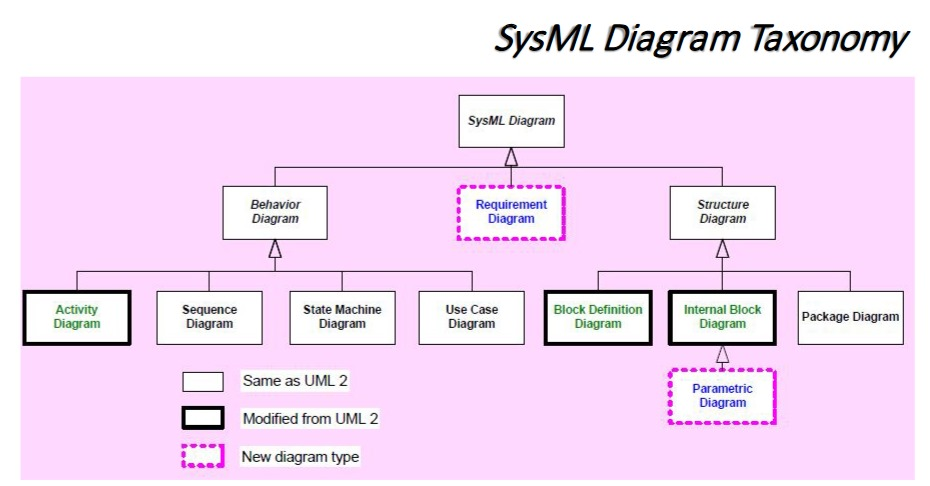
\includegraphics[width=0.5\textwidth]{diagrams.jpeg}
\end{figure}

\begin{figure}[h] % 'h' places the image approximately where it's included in the text
    \centering % Centers the image
    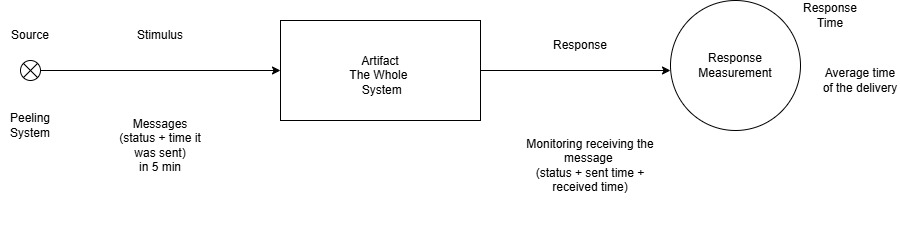
\includegraphics[width=0.5\textwidth]{scenario.jpeg}
\end{figure}
\vspace{12pt}
\end{document}